
% 完整编译方法 1 pdflatex -> bibtex -> pdflatex -> pdflatex
% 完整编译方法 2: xelatex -> bibtex -> xelatex -> xelatex
\documentclass[lang=cn,11pt,numbers]{elegantpaper}
\usepackage{float}
%% 去掉图标的冒号
\usepackage{caption}

\usepackage{url}%加入超链接  \href{http://v.youku.com/}{Youku video} 

\DeclareCaptionLabelSeparator{twospace}{\ ~}   %%这三条语句即可
\captionsetup{labelsep=twospace}
%%使用\upcite{}上标参考文献 
\newcommand{\upcite}[1]{\textsuperscript{\textsuperscript{\cite{#1}}}}


\title{《人人都是产品经理》读后感}
\author{0121710880223 - 软件工程1702 - 刘佳迎}

%\institute{\href{https://elegantlatex.org/}{Elegant\LaTeX{} 项目组}}

% 不需要版本信息,直接注释即可
%\version{0.07}
% 不需要时间信息的话,需要把 \today 删除。
\date{\today}
\geometry{a4paper,scale=0.8}
\usepackage{indentfirst}\setlength{\parindent}{2em}

\begin{document}

\maketitle

\section{序言}

《人人都是产品经理》是苏杰的第一本书。该书从产品经理的岗位职责和自我修养,需求的挖掘,项目的推进,团队的协作等方方面面描述,将
一个中国互联网蓬勃发展期的未来互联网帝国的优秀策划和建设者形象跃然纸上。全文共分三个板块分别使用思维导图+ \LaTeX 部分呈现《人人都是产品经理》读后感。详细的思维导图读书笔记详见链接
\href{https://github.com/ljyslyc/LATEX-model/blob/master/软件工程需求/figure/人人都是产品经理.pdf}{(https://github.com/ljyslyc/LATEX-model/blob/master/软件工程需求/figure/人人都是产品经理.pdf).} 
\begin{figure}[H]
	\centering
	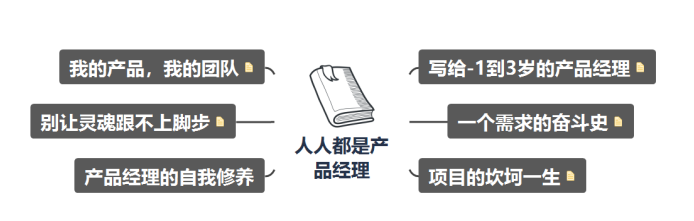
\includegraphics[width=12cm]{Snipaste_2019-09-19_19-31-46.png}
\end{figure}


\section{写给-1 -- 3岁的产品经理}

\begin{figure}[H]
	\centering
	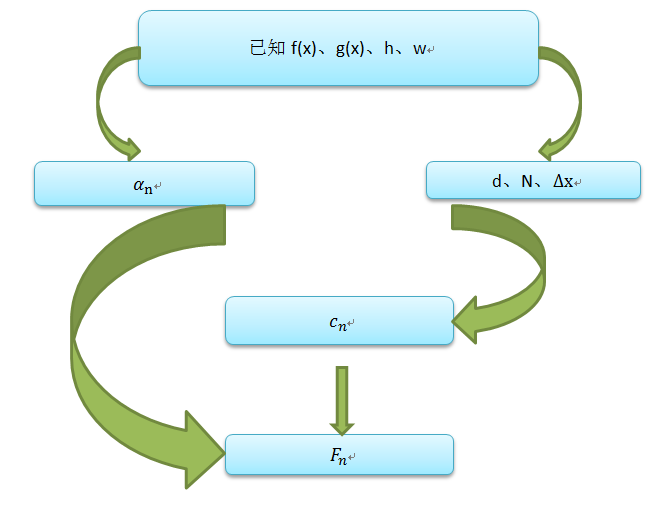
\includegraphics[width=12cm]{f1.png}
	\caption{ 写给-1 -- 3岁的产品经理 \label{fig:2}}
\end{figure}
产品经理指的是能够发新问题并描述清楚,转化为一个需求,进而转化为一个任务,争取到支持,发动一批人,并持续不断以主人翁的心态去跟踪,维护这个产物。
该书第一章主要从\figref{fig:2} 所示的三个部分展开描述。

相对于传统行业来讲,互联网行业对于产品经理的需求与日俱增。对于互联网行业来说,用户对产品的习惯并没有产生较大的
依赖性,这就要求产品经理先入为主,占领用户主导用户习惯。在产品的研发过程中,需求设计分析的细节也显得尤为重要。此外,由于
互联网软件行业的生命周期较短,产品的更新迭代时长往往只有几个周甚至几天,所以要在项目完成度和产品质量之间找到平衡。




\section{一个需求的奋斗史}

\begin{figure}[H]
	\centering
	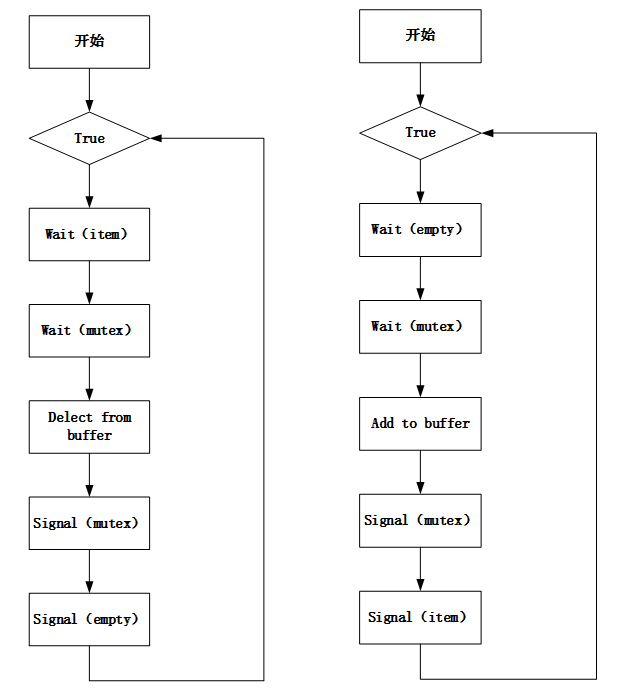
\includegraphics[width=12cm]{f2.png}
	\caption{ 《人人都是产品经理》思维导图 \label{fig:3}}
\end{figure}

产品广义上可以理解为解决某个问题的东西,而产品经理则是使用这个东西的人。书中从需求的获取,分析,转化,测试等几个角度描述了需求的曲折故事。
在我看来,产品经理需要具备的的很强的需求分析的能力,例如:
\begin{itemize}
\item \textbf{需求采集能力:} 把用户需求转化为产品需求,需要确定需求的基本属性,分析需求的商业价值,初评需求的实现难度,计算出它的性价比。
因为资源总是有限的,因此我们要懂的取舍。
\item \textbf{数据分析能力:}在对产品足够熟悉的基础上,先做出方向性的假设,再提取相应的数据并分析,得到一些现象, 最好是之前没发现的现象,然后尝试解释,接下来做用户调研修正解释,最终得出产品的最终发展方向。
\end{itemize}

\section{项目的坎坷一生}

\begin{figure}[H]
	\centering
	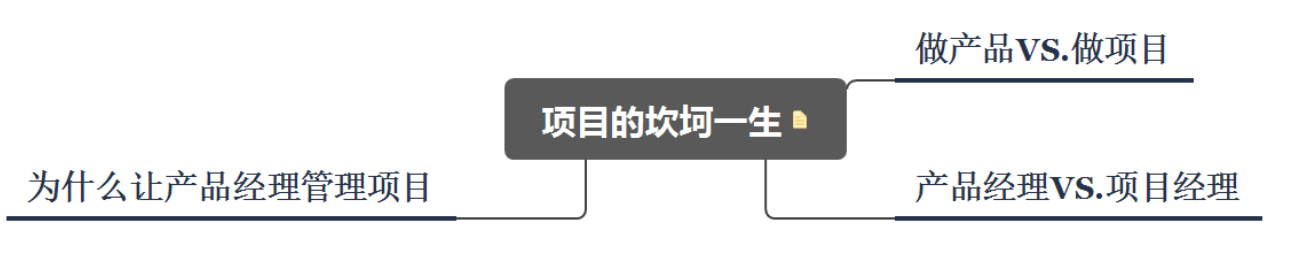
\includegraphics[width=12cm]{f3.png}
	\caption{ 《人人都是产品经理》思维导图 \label{fig:4}}
\end{figure}

做产品与做项目有很多不同点:从生命周期的角度来看,产品的生命周期相对较长,关注的市场品的整
个过程;而项目通常有特定的起止时间;
从具体要做的事情来看,产品需要不断地随着内外部变化进行修正;而
项目开始时已有明确目标,更注重计划与控制;
从产出物的角度来看,产品是可批量生产,相对通用的;而项目只进行
一次,通常是满足特定需求的。

而让产品管理项目,是希望能够在商业目标、项目资源、用户体验等各种限制条
件下取得平衡,解决目标不一致的问题
由谁来管理项目,并不是绝对的,要在产品功能特征满足用户需求以及项目如
期完成的冲突中取得平衡。


\nocite{*}
\bibliography{wpref}

\end{document}
